\documentclass[xcolor=x11names,compress]{beamer}
\usepackage[utf8]{inputenc}

%% packages
\usepackage{graphicx}
\usepackage{hyperref}
\usepackage{amsmath}
\usepackage{amssymb}
\usepackage{longtable}

%% hyperlinks
\hypersetup{
	colorlinks=true,
	linkcolor=blue,
	filecolor=blue,      
	urlcolor=blue,
	citecolor=blue
}

%% self-commands
\newcommand{\As}{\textit{Anabaena sp.}}
\newcommand{\Ss}{\textit{Synechocystic sp.}}
\newcommand{\Cs}{\textit{Chroococcidiopsis sp.}}
\newcommand{\Ct}{\textit{Chroococcidiopsis thermalis}}

\title{MRes: Eco-bioelectric Cell}
\author{PokMan Ho}
\date{16 January 2020}

\begin{document}

\begin{frame}
    \maketitle
\end{frame}

\begin{frame}{Computer Model Visualization}
    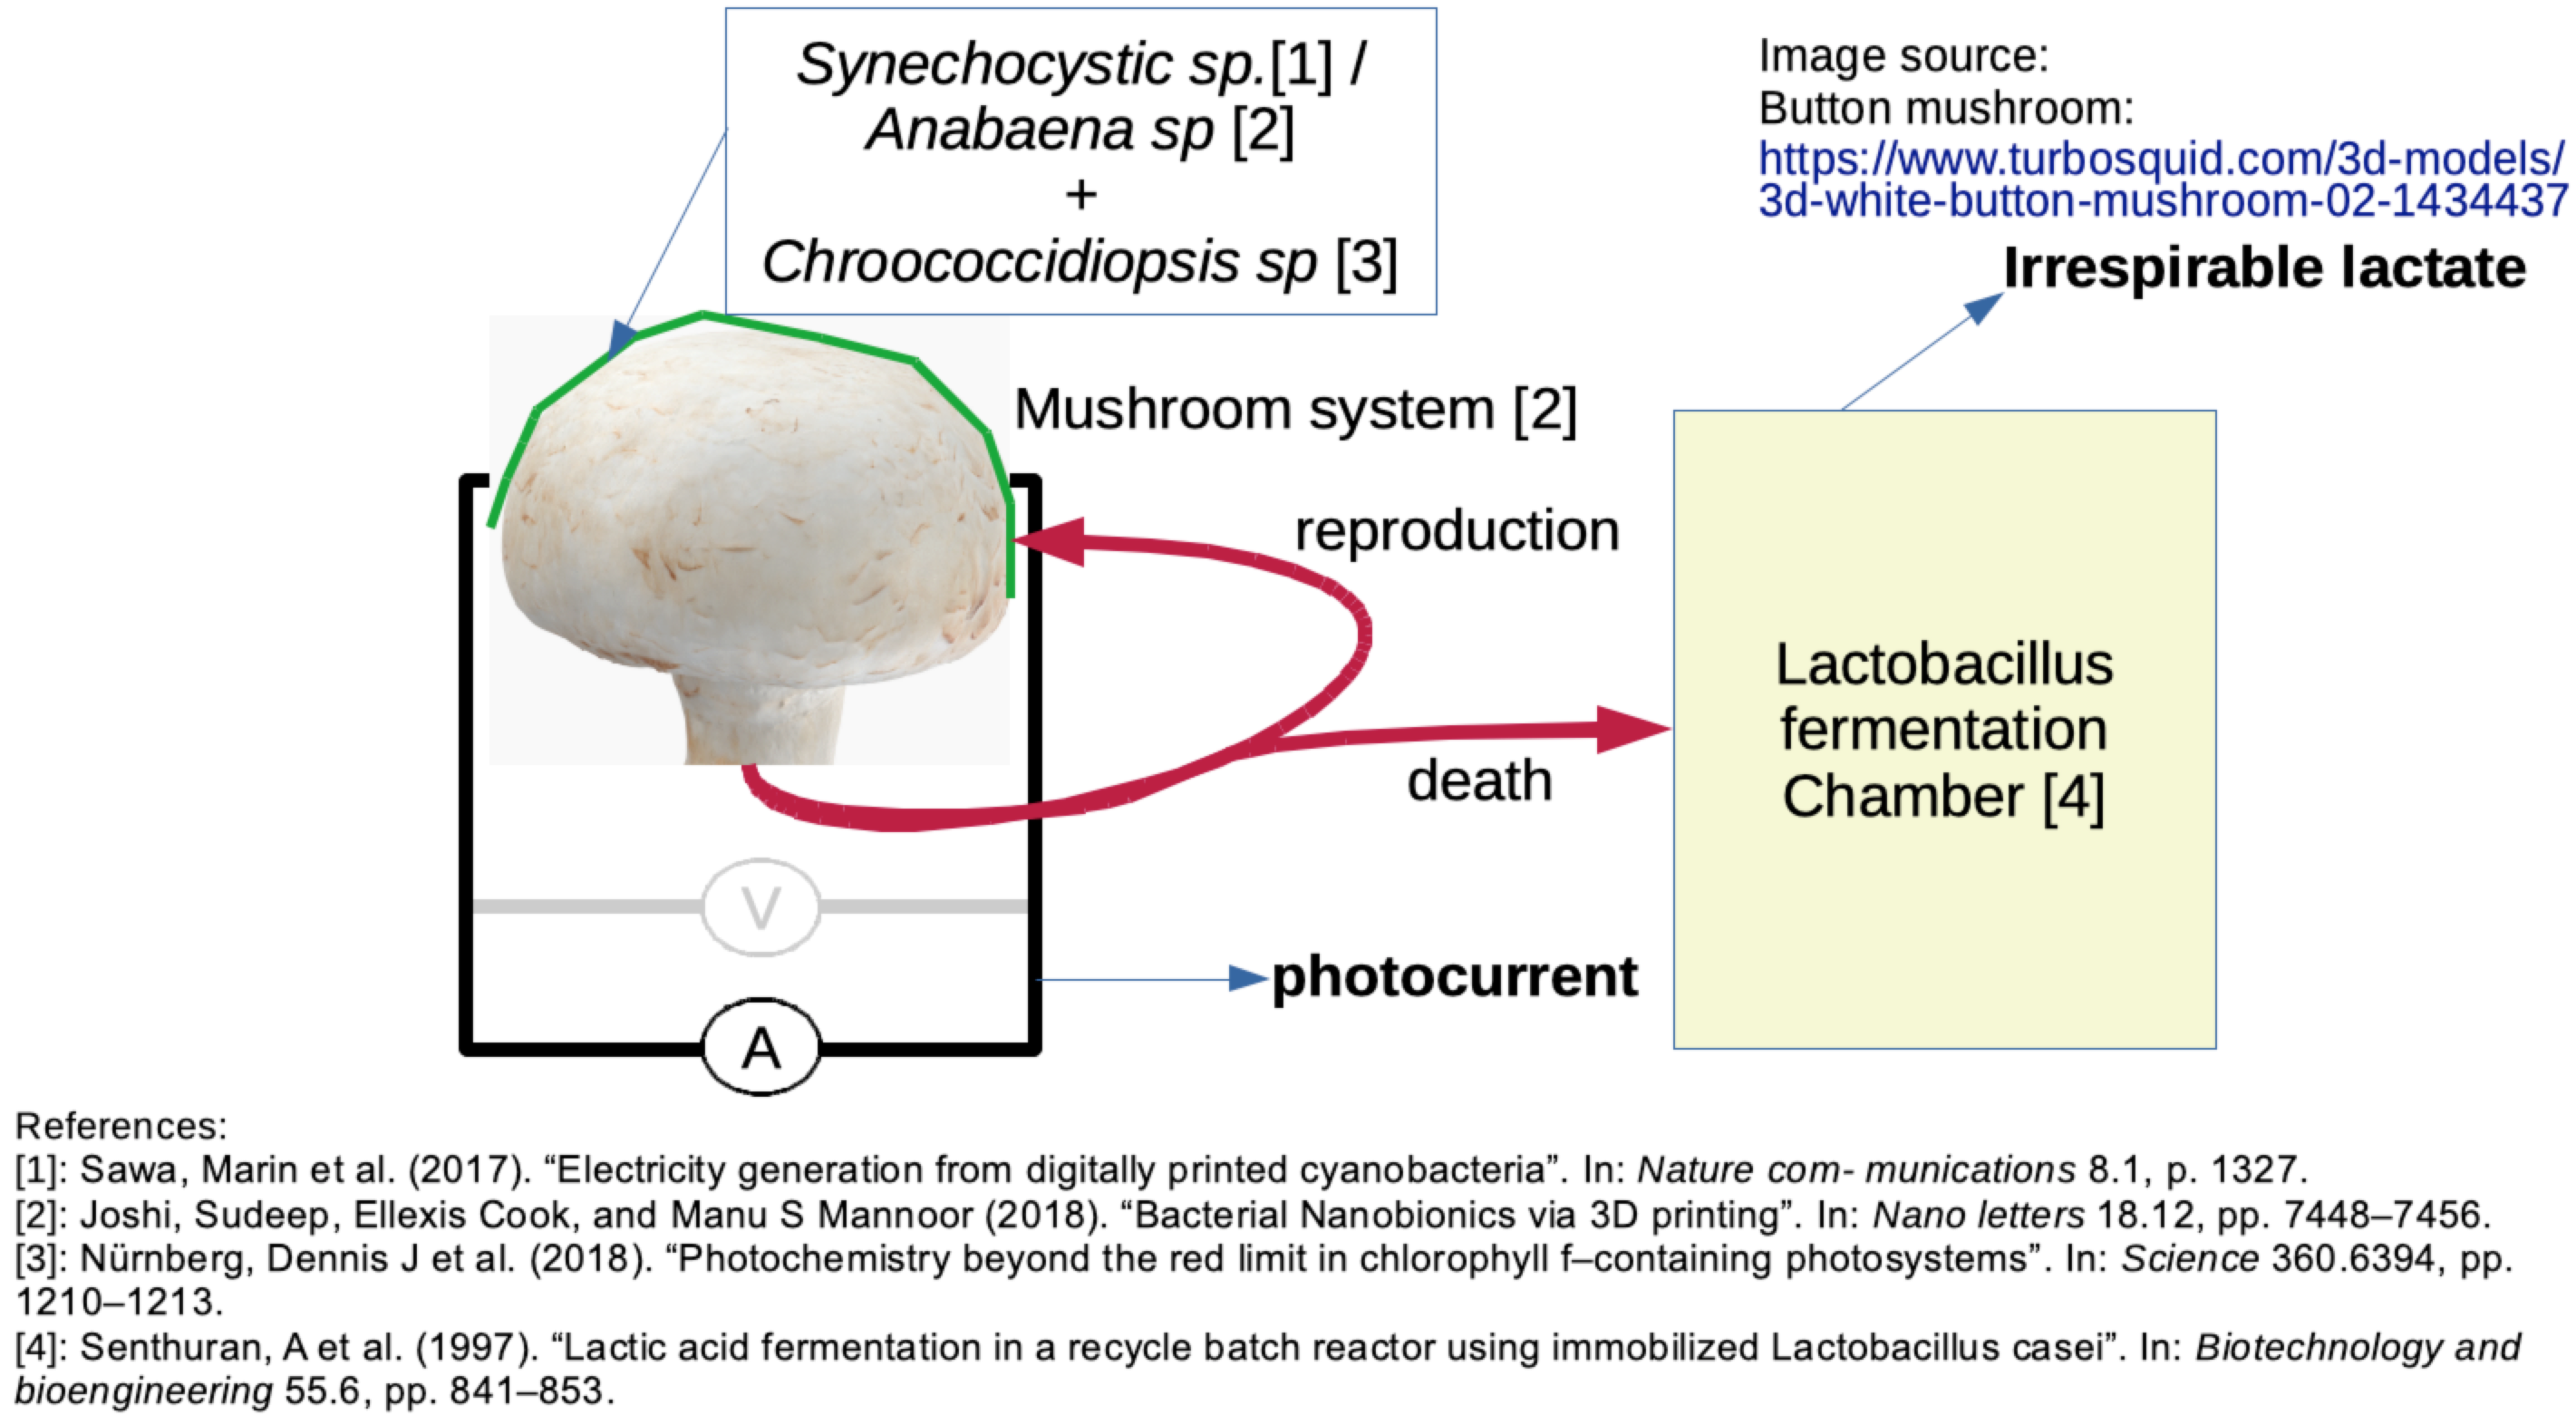
\includegraphics[width=\linewidth]{figure/proposed_model.png}
\end{frame}

\begin{frame}{Computer Model in Equations}
    pillar equation:
    \begin{equation}\label{eq:main}
        dp/dt = r_p [p] - k_{p1} [p][q]
    \end{equation}
    population growth rate:
    \begin{equation}\label{eq:growth}
        r_p = \dfrac{r_p|_{expt}}{P_p|_{expt}}\cdot P_p = \dfrac{r_p|_{expt}\cdot t_p|_{expt}}{J_p|_{expt}}\cdot\dfrac{J_p}{3600}
    \end{equation}
    competition coefficient:
    \begin{equation}\label{eq:compete}
        k_{p1} = \dfrac{P_q}{P_p + P_q}\cdot r_p = \dfrac{J_q J_p}{(J_p + J_q)\cdot3600}\cdot \dfrac{r_p|_{expt}\cdot t_p|_{expt}}{J_p|_{expt}}
    \end{equation}
    Overall equation (will be used in script):
    \begin{tabular}{rll}
        $\dfrac{dp}{dt}$ & = $[p]\cdot(r_p - k_{p1}[q]) = [p]\cdot r_p(1-\dfrac{P_q}{P_p + P_q}\cdot[q])$\\
         & = $[p]\cdot(\dfrac{r_p|_{expt}\cdot t_p|_{expt}}{J_p|_{expt}})\cdot\dfrac{J_p}{3600}\cdot(1-\dfrac{J_q[q]}{J_p + J_q})$
    \end{tabular}
\end{frame}

\begin{frame}{Data source for parameters}
    rate of population fluctuation:
    \begin{equation*}
        \dfrac{dp}{dt} = (\dfrac{r_p|_{expt}\cdot t_p|_{expt}}{3600\cdot J_p|_{expt}})(1-\dfrac{J_q[q]}{J_p + J_q})J_p[p]
    \end{equation*}
    \begin{longtable}{c|p{.8\linewidth}}
        term & description \\\hline
        $r_p|_{expt}$ & growth rate determined / reported in literature \\&\\
        $\dfrac{t_p|_{expt}}{J_p|_{expt}}$ & $\dfrac{1}{power}$ reported in literature \\&\\
        $\dfrac{J_p}{3600}$ & hourly solar energy (KJ/hr) with unit homogenization \\&\\
        $\dfrac{J_q[q]}{J_p + J_q}$ & population q living status description
    \end{longtable}
\end{frame}

\begin{frame}{Equation preliminary discussion}
    rate of population fluctuation:
    \begin{equation*}
        \dfrac{dp}{dt} = (\dfrac{r_p|_{expt}\cdot t_p|_{expt}}{3600\cdot J_p|_{expt}})(1-\dfrac{J_q[q]}{J_p + J_q})J_p[p]
    \end{equation*}
    Speculation:
    \begin{itemize}\itemsep10pt
        \item coexisting looks possible because interacting populations hindering each other
        \item solar cycle trend looks determining because it affect $J_p$ and $J_q$, changing instantaneous growth rate
        \item energy gained per cell by a population can only be max approximately equal to population
        \item initial population size might not be important
    \end{itemize}
\end{frame}

\begin{frame}{Progress}
    \begin{center}
        \begin{tabular}{l|lr}
            item & action / source & stage \\\hline
            model scripts & script &  d \\
            Global insolation & clean & d \\
            Global solar station & clean & d \\
            parameter numbers & collection & final \\
            model run & run & yet \\
            annual insolation cycle & validation & yet \\
            decade insolation cycle & validation & yet \\
            population flux & result & yet \\
            photocurrent & calculation & yet \\
            C-sequesteration & calculation & yet
        \end{tabular}\\
    \end{center}
\end{frame}

\begin{frame}{Timed steps}
    \begin{center}
        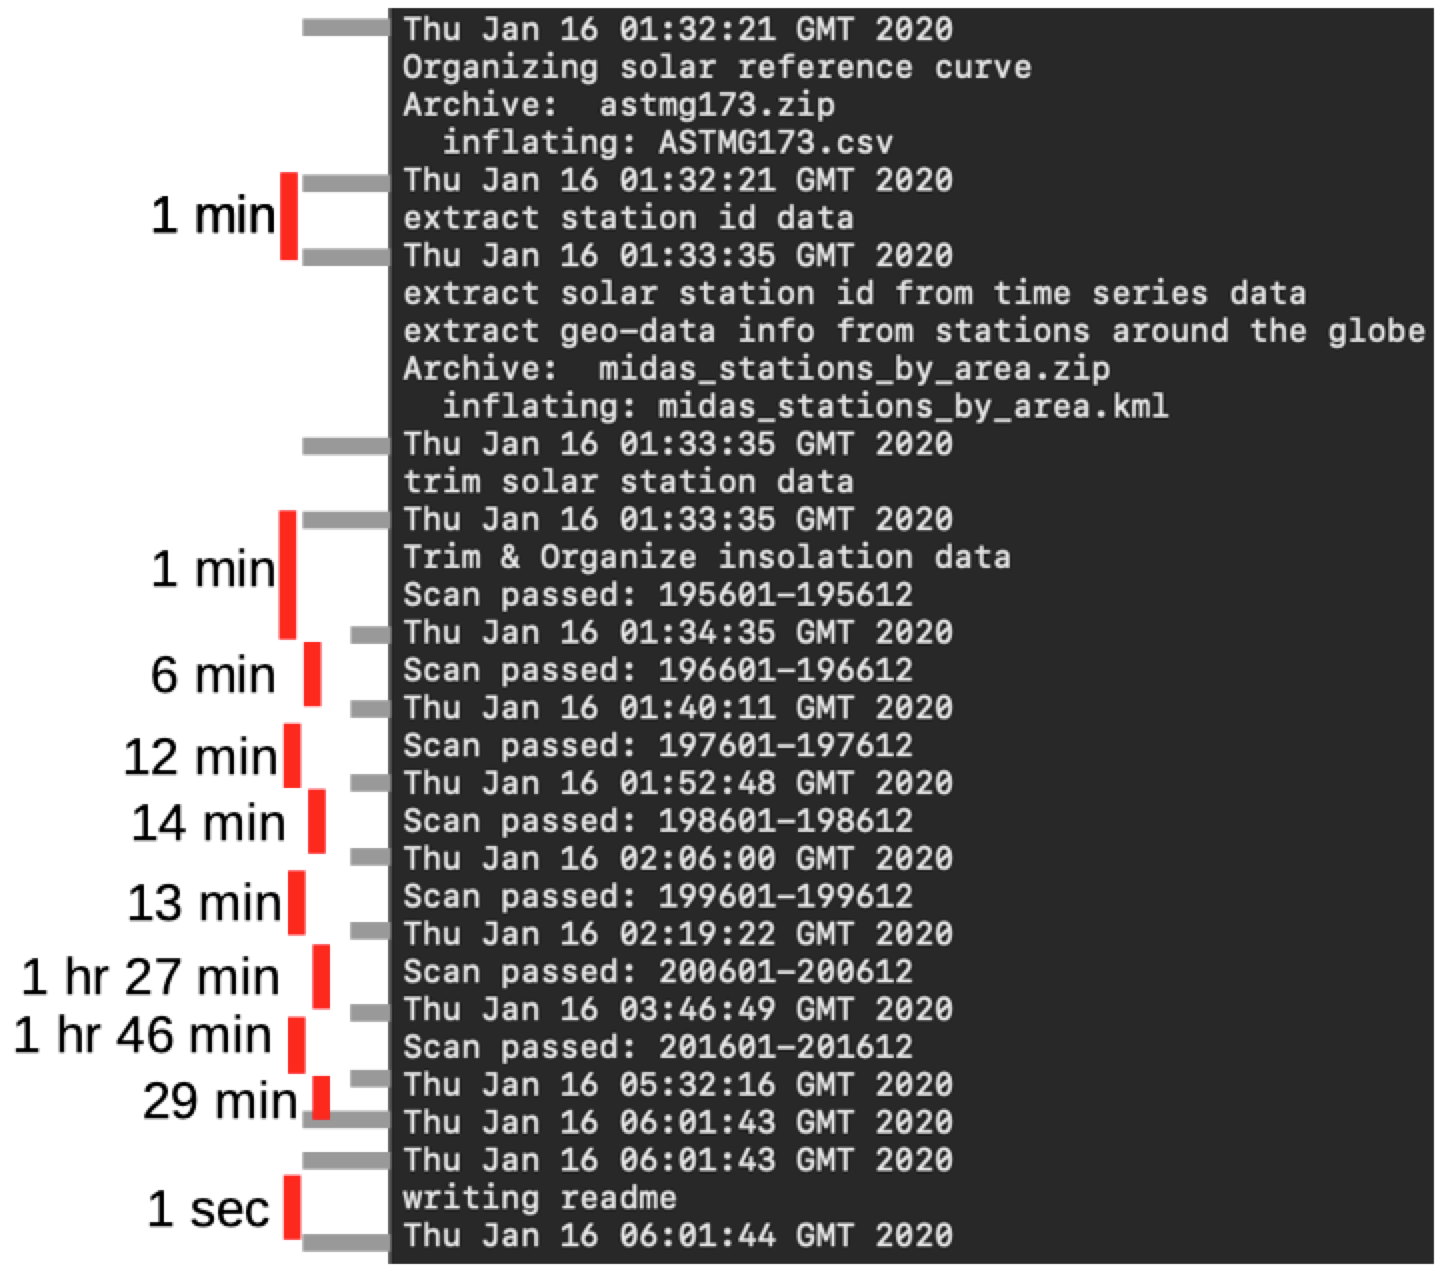
\includegraphics[width=.8\linewidth]{meeting/figure/timed_steps.png}\\
        \vspace{.3cm}
        - end -
    \end{center}
\end{frame}

\end{document}
